% main.tex
% header.tex
\documentclass[a4paper,11pt,twoside,ngerman,color]{book}
\usepackage[a4paper,left=3.5cm,right=2.5cm,bottom=3.5cm,top=3cm]{geometry}

\usepackage[german,english]{babel}

\usepackage[pdftex]{graphicx,color}
\usepackage{amsmath,amssymb,subfigure}
\usepackage{tikz}
\usepackage[miktex]{gnuplottex}
\usetikzlibrary{mindmap,trees,positioning}
\usetikzlibrary{arrows.meta,positioning}
\usetikzlibrary{calc}
\definecolor{darkertugreen}{RGB}{100,140,20}
\definecolor{tugreen}{RGB}{132,184,24}
\definecolor{cred}{RGB}{194,31,31}
\definecolor{cblue}{RGB}{31,61,194}


% Theorem-Umgebungen
\usepackage[amsmath,thmmarks]{ntheorem}

% Korrekte Darstellung der Umlaute
\usepackage[utf8]{inputenc}
\usepackage[T1]{fontenc}

% Algorithmen
\usepackage[plain,chapter]{algorithm}
\usepackage{algorithmic}
\usepackage{listings}
\lstset{language=C++}
\lstdefinestyle{customc}{
  belowcaptionskip=1\baselineskip,
  breaklines=true,
  frame=single,
  xleftmargin=\parindent,
  language=C++,
  showstringspaces=false,
  basicstyle=\footnotesize\ttfamily,
  keywordstyle=\bfseries\color{green!40!black},
  commentstyle=\itshape\color{white!40!black},
  identifierstyle=\color{blue},
  stringstyle=\color{purple!60!black},
  morekeywords={DATA_TYPE},
}
\lstset{escapechar=@,
	style=customc,
	emph={pragma,HLS,LOOP,FLATTEN},
  	emphstyle={\color{purple!60!black}},
  	emph={[2]f},
  	emphstyle={[2]\color{black}},
  	emph={[3]FEATURE_COUNT,BATCH_SIZE},
  	emphstyle={[3]\bfseries\color{orange!60!black}},
  	emph={[4]predict,learn},
  	emphstyle={[4]\bf\color{black}}
}

\usepackage{enumerate}


% Bibtex deutsch
\usepackage{bibgerm}

% URLs
\usepackage{url}

% Caption Packet
\usepackage[margin=0pt,font=small,labelfont=bf]{caption}
% Gliederung einstellen
%\setcounter{secnumdepth}{5}
%\setcounter{tocdepth}{5}

% Theorem-Optionen %
\theoremseparator{.}
\theoremstyle{change}
\newtheorem{theorem}{Theorem}[section]
\newtheorem{satz}[theorem]{Satz}
\newtheorem{lemma}[theorem]{Lemma}
\newtheorem{korollar}[theorem]{Korollar}
\newtheorem{proposition}[theorem]{Proposition}
% Ohne Numerierung
\theoremstyle{nonumberplain}
\renewtheorem{theorem*}{Theorem}
\renewtheorem{satz*}{Satz}
\renewtheorem{lemma*}{Lemma}
\renewtheorem{korollar*}{Korollar}
\renewtheorem{proposition*}{Proposition}
% Definitionen mit \upshape
\theorembodyfont{\upshape}
\theoremstyle{change}
\newtheorem{definition}[theorem]{Definition}
\theoremstyle{nonumberplain}
\renewtheorem{definition*}{Definition}
% Kursive Schrift
\theoremheaderfont{\itshape}
\newtheorem{notation}{Notation}
\newtheorem{konvention}{Konvention}
\newtheorem{bezeichnung}{Bezeichnung}
\theoremsymbol{\ensuremath{\Box}}
\newtheorem{beweis}{Beweis}
\theoremsymbol{}
\theoremstyle{change}
\theoremheaderfont{\bfseries}
\newtheorem{bemerkung}[theorem]{Bemerkung}
\newtheorem{beobachtung}[theorem]{Beobachtung}
\newtheorem{beispiel}[theorem]{Beispiel}
\newtheorem{problem}{Problem}
\theoremstyle{nonumberplain}
\renewtheorem{bemerkung*}{Bemerkung}
\renewtheorem{beispiel*}{Beispiel}
\renewtheorem{problem*}{Problem}

% Algorithmen anpassen %
\renewcommand{\algorithmicrequire}{\textit{Eingabe:}}
\renewcommand{\algorithmicensure}{\textit{Ausgabe:}}
\floatname{algorithm}{Algorithmus}
\renewcommand{\listalgorithmname}{Algorithmenverzeichnis}
\renewcommand{\algorithmiccomment}[1]{\color{grau}{// #1}}

% Zeilenabstand einstellen %
\renewcommand{\baselinestretch}{1.25}
% Floating-Umgebungen anpassen %
\renewcommand{\topfraction}{0.9}
\renewcommand{\bottomfraction}{0.8}
% Abkuerzungen richtig formatieren %
\usepackage{xspace}
\newcommand{\vgl}{vgl.\@\xspace} 
\newcommand{\zB}{z.\nolinebreak[4]\hspace{0.125em}\nolinebreak[4]B.\@\xspace}
\newcommand{\bzw}{bzw.\@\xspace}
\newcommand{\dahe}{d.\nolinebreak[4]\hspace{0.125em}h.\nolinebreak[4]\@\xspace}
\newcommand{\etc}{etc.\@\xspace}
\newcommand{\evtl}{evtl.\@\xspace}
\newcommand{\ggf}{ggf.\@\xspace}
\newcommand{\bzgl}{bzgl.\@\xspace}
\newcommand{\so}{s.\nolinebreak[4]\hspace{0.125em}\nolinebreak[4]o.\@\xspace}
\newcommand{\iA}{i.\nolinebreak[4]\hspace{0.125em}\nolinebreak[4]A.\@\xspace}
\newcommand{\sa}{s.\nolinebreak[4]\hspace{0.125em}\nolinebreak[4]a.\@\xspace}
\newcommand{\su}{s.\nolinebreak[4]\hspace{0.125em}\nolinebreak[4]u.\@\xspace}
\newcommand{\ua}{u.\nolinebreak[4]\hspace{0.125em}\nolinebreak[4]a.\@\xspace}
\newcommand{\og}{o.\nolinebreak[4]\hspace{0.125em}\nolinebreak[4]g.\@\xspace}
\newcommand{\oBdA}{o.\nolinebreak[4]\hspace{0.125em}\nolinebreak[4]B.\nolinebreak[4]\hspace{0.125em}d.\nolinebreak[4]\hspace{0.125em}A.\@\xspace}
\newcommand{\OBdA}{O.\nolinebreak[4]\hspace{0.125em}\nolinebreak[4]B.\nolinebreak[4]\hspace{0.125em}d.\nolinebreak[4]\hspace{0.125em}A.\@\xspace}

% Leere Seite ohne Seitennummer, naechste Seite rechts
\newcommand{\blankpage}{
 \clearpage{\pagestyle{empty}\cleardoublepage}
}

% Keine einzelnen Zeilen beim Anfang eines Abschnitts (Schusterjungen)
\clubpenalty = 10000
% Keine einzelnen Zeilen am Ende eines Abschnitts (Hurenkinder)
\widowpenalty = 10000 \displaywidowpenalty = 10000
% EOF

\begin{document}
\selectlanguage{german}
\begin{titlepage}
\definecolor{TUGreen}{rgb}{0.517,0.721,0.094}
\vspace*{-2cm}
\newlength{\links}
\setlength{\links}{-1.5cm}
\sffamily
\hspace*{\links}
\begin{minipage}{12.5cm}

\includegraphics[width=8cm]{bilder/tud_logo_rgb}
%\hspace*{-0.25cm} \textbf{TECHNISCHE UNIVERSIT"AT DORTMUND}\\
%\hspace*{-1.2cm} \rule{5mm}{5mm} \hspace*{0.1cm} FACHBEREICH INFORMATIK\\
\end{minipage}

\vspace*{4cm}

\hspace*{\links}
\hspace*{-0.2cm}
\begin{minipage}{9cm}
\large
\begin{center}
{\Large Bachelorarbeit} \\
\vspace*{1cm}
\textbf{Optimierung von logistischer Regression auf FPGAs} \\
\vspace*{1cm}
Moritz Sliwinski\\
% \vspace*{1cm}
Februar 2020
\end{center}
\end{minipage}
\normalsize
\vspace*{5.5cm}

% \hspace*{\links}

\vspace*{2.1cm}

\hspace*{\links}
\begin{minipage}[b]{5cm}
% \normalsize
\raggedright
Gutachter: \\
Prof. Dr. Katharina Morik \\
Sebastian Buschjäger \\
\end{minipage}

\vspace*{2.5cm}
\hspace*{\links}
\begin{minipage}[b]{8cm}
% \normalsize
\raggedright
Technische Universit"at Dortmund \\
Fakult"at f"ur Informatik\\
Lehrstuhl für Künstliche Intelligenz (LS-8)\\
https://www-ai.cs.tu-dortmund.de
\end{minipage}
%%%%%%%%%%%%%%%%%%%%%%%%%%%%%%%%%%%%%%%%%%%%%%%%%%
% bei Kooperation mit anderen Lehrstuehlen,
% sonst weglassen
\begin{minipage}[b]{8cm}
% \normalsize
\raggedleft
\end{minipage}
%%%%%%%%%%%%%%%%%%%%%%%%%%%%%%%%%%%%%%%%%%%%%%%%%%

\end{titlepage}

\blankpage
\pagenumbering{roman}
\tableofcontents
\cleardoublepage
\pagenumbering{arabic}
% Kapitel
% einleitung.tex
\chapter{Einleitung}
\section{Motivation und Hintergrund}
Maschinelles Lernen und Vorhersagen werden immer mehr in unser Leben integriert. Hierbei entsteht zum einen der Anspruch an variable, nicht statische Systeme, zum anderen die Notwendigkeit kompakter und energieeffizienter Lösungen.\\
Aufgrund der immer weiter wachsenden Datenmengen stoßen herkömmliche Central Processing Units (CPUs) mittlerweile an Ihre Grenzen, denn durch materialbedingte Limitierung kann ihre Rechenkapazität so gut wie nicht mehr erhöht werden. Daher geht man dazu über, Mehrkernprozessoren zu entwickeln, die ihre Geschwindigkeit über parallele Threads erreichen. Diese haben jedoch einen vergleichsweise hohen Energieverbrauch.\\
Field Programmable Gate Arrays (FPGAs) bieten in diesem Zusammenhang einen guten Kompromiss zwischen Flexibilität in der Programmierbarkeit und Energieeffizienz. Der Vorteil der FPGAs zeigt sich in der deutlich höheren Parallelität gegenüber CPUs, sodass trotz der geringeren Taktfrequenz eine große Menge an Daten schnell verarbeitet werden kann.\\
Die logistische Regression ist für die Optimierung auf FPGAs in dem Sinne gut geeignet, da sie eine einfache Art von neuronalem Netz darstellt und somit gut in der FPGA-Logik darstellbar ist. Sie weist zum Beispiel durch Datenparallelität bzw. Parallelisierung von Batches, Feature- oder Hyperparameter-Berechnung eine hohe Parallelisierbarkeit auf.\\\\
Moderne FPGAs können über die PCIe-Schnittstelle als Co-Prozessor in ein System eingebunden werden, sodass deren Parallelität und Energieeffizienz ausgenutzt werden können. Dank des hohen Durchsatzes der Schnittstelle muss hierbei nicht auf eine komplexe variable Vorbereitung der Daten durch die CPU im laufenden Betrieb verzichtet werden.\\
Die Motivation zur Nutzung von FPGAs besteht darin, dass sie Energieeffizienz und Parallelität miteinander kombinieren. Sie bieten einen guten Kompromiss zur Nutzung von Graphics Processing Units (GPUs), denn diese weisen zwar eine noch höhere Parallelisierungseigenschaft auf, benötigen aber auch deutlich mehr Energie, bis zu 20x mehr allein im Idle-Zustand \cite{GPU}. Aufgrund dessen werden GPUs in der Arbeit nicht weiter behandelt.

\section{Aufbau der Arbeit}
In Kapitel 2 werden zunächst der Aufbau und die Funktionsweise von FPGAs erläutert. Es wird auf die technischen Besonderheiten und die Funktion der Einzelnen Hardwarebausteine eingegangen. Außerdem wird der Konfigurationsablauf zur Programmierung des FPGAs erklärt und seine Eigenschaften mit denen von anderen Hardwarekomponenten verglichen.\\\\
Im 3. Kapitel erörtern wir die Zusammensetzung der Logistischen Regression. Ihre Funktion als Lernfunktion wird detailliert beschrieben und mit Hilfe des Gradientenabstiegsverfahrens wird eine Updatefunktion für Koeffizienten hergeleitet. Es folgt eine Vorstellung verschiedener Regularisierungsmethoden sowie deren Einbindung in in die Updatefunktion.\\\\
in Kapitel 4 werden die Implementierten Programme dargestellt und der Code erörtert. Man geht auf die Probleme der Entwicklung für den FPGA-Code und den Hostanwedungs-Code ein, sowie dessen Grenzen in der Anwendung.\\
Kapitel 5 fast die Ergebnisse von Experimenten mit dem FPGA zusammen. Es werden beispielhaft Daten ausgewertet und Trainingsergebnisse vorgestellt.Auch eine Analyse der Geschwindigkeit im Vergleich zu einer CPU werden behandelt. \\Im 6. Kapitel wird das Fazit aus den behandelten Themen und Ergebnissen dieser Arbeit gezogen. Es werden Empfehlungen für weitere, tiefer gehende Implementierungen und Experimente gegeben, die zum Teil aus Zeit- und Aufwandstechnischer Sicht in der Arbeit nicht behandelt werden.
\section{Verwandte Arbeiten}
Es gibt bereits einige Arbeiten zu dem Thema logistische Regression auf FPGAs die sich mit der Energie- und Geschwindigkeitsoptimierung auseinandersetzen.
Wienbrandt et al. benutzen ein FPGA mit logistischer Regression in \cite{WIENB} und zeigen, dass ein hybrides System aus GPU und FPGA einen Speedup von über 1500 gegenüber einem PLINK hat. Allerdings benutzten sie zum Einen eine GPU mit einem Energieverbrauch von 300 Watt \cite{P100}, was im Gegensatz zu einem einzelnen Artix 7 FPGA mit einem Verbrauch von ca. 5 Watt \cite{WAT} sehr hoch ist, und zum anderen werden in dem Artikel keine Werte eines FPGAs als einzelnes System gemessen.
Es gibt bereits eine Implementierung von InAccel von logistischer Regression auf FPGAs \cite{ACC} die sich jedoch vor allem auf die Nutzung in vernetzten Systemen und Kubernetes bezieht. Zum Beispiel werden in der Implementierung alle benötigten Ressourcen für die maximalen Eingabegrößen (64 Klassen und 2047 Features) auf jedem FPGA reserviert,
was vor allem für Trainingsdaten mit deutlich weniger Features eine unnötige Speicherausnutzung bedeutet. Es wird mit float8 bzw float16 gearbeitet, sodass eine Implementierung mit Fixkommazahlen eine noch etwas bessere Performance erzielen könnte. Die Implementierung nutzt zudem keine PCIe Schnittstelle und programmiert die FPGAs während des Hostprozess mit einem Bitstream jedes mal erneut.
% fpga.tex
\chapter{FPGAs}
Die Arbeit befasst sich mit der Implementierung und Optimierung von Logistischer Regression auf FPGAs. Deshalb wird zunächst der allgemeine Aufbau dieser beschrieben. Dann folgt eine Einführung in die Konfiguration des FPGAs, wobei zum einen auf den typischen Ablauf, zum anderen auf die verwendeten Programme eingegangen wird. Abschließend wird die verwendete Hard- und Software aufgeführt.
\section{Allgemeiner Aufbau von FPGAs}
Field Programmable Gate Arrays (FPGAs) sind Integrierte Schaltkreise (IC) in die eine logische Schaltung programmiert werden kann. Die ICs bestehen aus I/O-Blöcken, Programmierbaren Logikblöcken (Configurable Logig Blocks, kurz CLB) und weiteren Bestandteilen wie zum Beispiel DSP-Slices, BRAM-Blöcken, Multipliziereinheiten oder Taktgeneratoren welche durch Datenpfade zu einer Matrix miteinander verbunden sind (Siehe Abbildung 2.1).\\
\begin{figure}[ht]
	\begin{minipage}[b]{.4\linewidth}
  		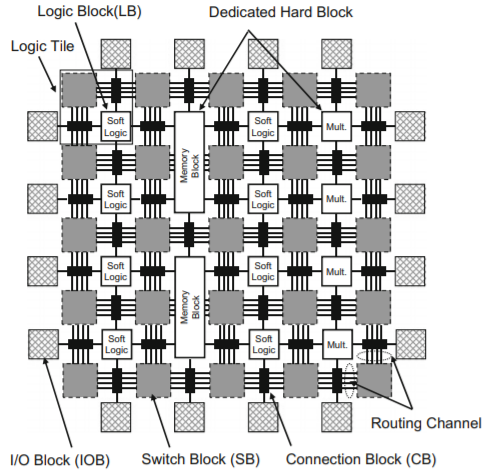
\includegraphics[scale=0.7]{bilder/matrix}
  		\caption{Aufbau eines IC, die grauen Schaltblöcke (SB) sind die konfigurierbaren Datenpfade}
  	\end{minipage}
  	\hspace{.1\linewidth}% Abstand zwischen Bilder
  	\begin{minipage}[b]{.4\linewidth}
  		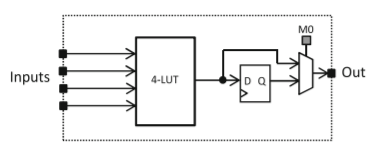
\includegraphics[scale=0.70]{bilder/clp}
		\caption{Schematische Darstellung eines CLB\\
		}
	\end{minipage}
	
\end{figure}
Die Pfade können je nach Bedarf geschaltet werden. Die CLPs selbst bestehen aus einem 1 Bit Flip-Flop und einer programmierbaren Wahrheitstabelle. Über diese lassen sich die logischen Funktionen konfigurieren\cite{TOSU}. Ein schematischer Aufbau ist in Abbildung 2.2 zu sehen. Dieser Aufbau ist typisch für ein FPGA der Marke Xilinx und nicht allgemein für andere Hersteller gültig. Da in dieser Arbeit (wie in Kapitel 2.3 beschrieben) ein FPGA der Marke Xilinx benutzt wird, wird auch dessen Hardwarekonfiguration zugrunde gelegt.\\\\
Die Programmierung ist in diesem Fall vergleichbar mit einer Schalttabelle, welche bestimmt wie die physikalischen Bausteine miteinander verbunden werden sollen. Anders als bei Application-Specific Integrated Circuits
(ASICs), dessen Funktion bereits bei der Produktion festgelegt werden, können FPGAs vom Benutzer selbst Konfiguriert werden. \newpage 
Dies geschieht jedoch im Gegensatz zu Mikroprozessoren nicht während, sondern vor Inbetriebnahme des Chips. Zwar ist es bei
einigen wenigen Herstellern von FPGAs mittlerweile möglich, diese auch wärend des laufenden Betriebs zu konfigurieren (partielle Rekonfiguration), aber das ist mit einer höheren
Komplexität der zu konfigurierenden Logik verbunden.\\
Durch die Konfigurierbarkeit des FPGAs ergeben sich bautechnisch bedingt einige Nachteile gegenüber den ASICs. FPGAs sind annäherungsweise 20 bis 35 mal größer und zwischen 3 und 4 mal langsamer als eine vergleichbare ASCI Implementierung. Außerdem verbrauchen sie dynamisch circa 10 mal mehr Energie \cite{KURO}.
%Vergleich mit CPU und GPU
Damit sind sie deutlich ineffizienter als ASICs. Der große Vorteil ergibt sich hier aus der Konfigurierbarkeit, denn ASICs sind nach der Produktion nicht mehr veränderbar. Besonders in Bereichen die eine hohe Flexibilität verlangen ist es vor allem Kosteneffizienter FPGAs zu benutzen, denn die Produktion von ASICs ist mit großen zeitlichen und finanziellen Investitionen verbunden\cite{KUTERO}.
\section{Konfiguration und Ablauf}
Wie das "`Field Programmable"' im Namen schon besagt ist es möglich nach der Fabrikation des FPGA Funktionen in diese "`in the field"', also im praktischen Einsatz zu programmieren \cite{KUTERO}. Um seine Funktion zu verändern muss das FPGA neu Konfiguriert werden. Dies geschieht durch einen sogenannten "`Bitstream"', eine Sequenz von einzelnen Bits. In Abbildung 2.3 zeigt sich der Ablauf zur Generierung einen solchen Bitstreams für ein FPGA der Marke Xilinx.\newpage
\begin{figure}
\begin{tikzpicture}[
    mynode/.style={rectangle,rounded corners,draw=black,
    top color=tugreen!50, bottom color=tugreen!50,thick, inner sep=1em, minimum size=3em,text centered},
    plus/.style={circle,draw=black,
    top color=tugreen, bottom color=tugreen,thick, text centered},
    myarrow/.style={-{Stealth}, shorten >=1pt, thick},
    myarrowdot/.style={-{Stealth}, shorten >=1pt, thick, dashed},
    mydots/.style={dashed, thick},
    line/.style={thick},
    inpnode/.style={},
    dotsred/.style={dashed, thick, color=cred},
    dotsblue/.style={dashed, thick, color=cblue}
]
\node[text width=2cm ,text centered] (dm) {Code in\\ Hochsprache};
\node[mynode, right=1cm of dm, text width=2.2cm](csim){Simulation Hochsprache};
\node[above=1.25cm of dm] (dummydm) {};
\node[mynode, right=1cm of csim, text width=2.2cm](hls){High-Level\\ Synthese};  
\node[mynode, right=1cm of hls, text width=2.2cm](cosim){HS/RTL\\ Kosimulation }; 
\node[mynode, below=2cm of cosim, text width=2.2cm](bd){Blockdesign\\ };
\node[above=1cm of hls] (dummyhls) {};
\node[below=0.8cm of hls] (dummyhlsb){};
\node[right=3.35cm of dummyhlsb](dummycosim){};
\node[mynode, left=1cm of bd, text width=2cm](sim){Simulation};  
\node[mynode, left=1cm of sim, text width=2cm](synth){Synthese};  
\node[mynode, left=1cm of synth, text width=2cm](impl){Implemen- tierung};     
\node[above=1cm of hls](space){};
\node[below=1cm of impl, text width=2.2cm, ,text centered](bs){Fertiger\\ Bitstream};
\node[above=1cm of cosim, text width=2.2cm, ,text centered](rtl){Code in HDL};


\node[left=0.1cm of dm](ring1r){};
\node[above=3cm of ring1r](ring2r){};
\node[right=1cm of ring2r,color=cred](ring2ar){Vivado HLS};
\node[right=11.3cm of ring2ar](ring3r){};
\node[below=5.23cm of ring3r](ring4r){};
\node[below=2cm of ring1r](ring7r){};
\node[above=0.03cm of ring7r](ring1b){};
\node[right=14.6cm of ring1b](ring2b){};
\node[below=4.5cm of ring2b](ring3b){};
\node[below=4.5cm of ring1b](ring4b){};
\node[right=4cm of ring4b, color=cblue](ring5b){Vivado Desing Suite};

\draw[mydots]  (dm.north) -- (dummydm.south);
\draw[mydots]  (dummydm.east) -- (dummyhls.west);
\draw[myarrowdot]  (dummyhls.south) -- (hls.north);
\draw[myarrow] (dm.east) -- (csim.west);
\draw[myarrow] (csim.east) -- (hls.west);
\draw[myarrow] (hls.east) -- (cosim.west);
\draw[myarrow] ($(cosim.south)!0.25!(cosim.south east)$) -- ($(bd.north)!0.25!(bd.north east)$);
\draw[myarrowdot] (dummycosim) -- ($(bd.north)!0.25!(bd.north west)$);
\draw[mydots] (hls.south) -- (dummyhlsb);
\draw[mydots] (dummyhlsb) -- (dummycosim);
\draw[myarrow] (bd.west) -- (sim.east);
\draw[myarrow] (sim.west) -- (synth.east);
\draw[myarrow] (synth.west) -- (impl.east);
\draw[myarrow] (impl.south) -- (bs.north);
\draw[myarrowdot] (rtl.south) -- (cosim.north);
\draw[dotsred] (ring1r) -- (ring2r);
\draw[dotsred] (ring2r) -- (ring2ar);
\draw[dotsred] (ring2ar) -- (ring3r);
\draw[dotsred] (ring3r) -- (ring4r);
\draw[dotsred] (ring4r) -- (ring7r);
\draw[dotsred] (ring7r) -- (ring1r.north);
\draw[dotsblue] (ring1b) -- (ring2b);
\draw[dotsblue] (ring2b) -- (ring3b);
\draw[dotsblue] (ring3b) -- (ring5b);
\draw[dotsblue] (ring5b) -- (ring4b);
\draw[dotsblue] (ring4b) -- (ring1b);
\end{tikzpicture}
\caption{Konfigurationsablauf eines Xilinx-FPGAs}
\end{figure}
Historisch bedingt wurde die RTL (Register Transfer Level) für einen Xilinx-FPGA grundsätzlich in einer HDL (Hardware Definition Language) programmiert. Erst seit 2012 gibt es die Tools Vivado Design Suite und Vivado HLS mit denen zusätzlich eine Programmierung in einer Hochsprache, bei Xilinx sind C/C++,  möglich ist. Somit ist diese Möglichkeit noch relativ neu und nicht so weit verbreitet wie die Benutzung von HDLs \cite{XIL4}.
Auch wenn der direkte Ansatz zu effizienteren Designs führen kann ist er doch mit erheblichem Mehraufwand verbunden. Vor allem der geringere Programmieraufwand in C++ gegenüber einem nicht signifikantem Leistungsverlust ist ausschlaggebend dafür, dass dieser Ansatz in der Arbeit nicht weiter behandelt wird, jedoch einen Ausblick auf weitere Verbesserungsmöglichkeiten bietet.\\\\
In dem von Xilinx für die High-Level Synthese vorgesehenem Workflow programmiert man nun zunächst die geplante Anwendung/Funktion in einer beliebigen Hochsprache, zum Beispiel BSV in Bluespec oder MaxJ in MaxCompiler. Die am häufigsten verwendete Sprache ist jedoch C oder C++, wie auch in diesem Fall mit Vivado HLS\cite{NASI}.\\\\ Dann folgt eine Simulation des Programms um dessen Tauglichkeit für eine FPGA Konfiguration zu prüfen. Hierbei wird die Funktionalität des eingegebenen Codes getestet, noch bevor es in die HDL übersetzt wird. Dieser Schritt ist optional, jedoch sehr hilfreich, denn die High-Level Synthese von Vivado HLS nimmt sowohl Zeit als auch Ressourcen auf dem Hostrechner in Anspruch und unterstützt zudem nicht alle Besonderheiten und Datentypen von C++. Es können zum Beispiel keine Arrays mit variabler (zur Laufzeit definierter) Länge instanziiert oder rekursive Funktionen verwendet werden. Außerdem werden Anfragen an das System nicht unterstützt und die Hauptfunktion muss die gesamte Funktionalität des Designs enthalten \cite{XIL2}.\\Nun wird mit der High-Level Synthese ein Programm in einer HDL, in diesem Fall VHDL oder Verilog, erstellt.\\
Man kann nun die Hochsprache und die RTL nebeneinander (ko-) simulieren, um das Verhalten der HLS zu verifizieren. Auch dieser Schritt ist optional und dient der frühen Fehlerfindung. Er führt eine erneute Kontrolle der Funktionalität durch um auszuschließen, dass bei der Übersetzung unerwünschte oder ungeplante Verhaltensweisen auftreten. \\
Nach diesem Schritt wird das RTL-Design als IP (Intellectual Property) exportiert und mit der Vivado Design Suite von Xilinx weiter bearbeitet. Zusammen mit IP-Blöcken von Xillinx und Drittanbietern erstellt man nun ein funktionstüchtiges Design, indem man die Ein- und Ausgänge der Blöcke sinnvoll miteinander verknüpft.\\ Das erstellte Projekt geht jetzt in den Simulaionsschritt, bei dem das echte Verhalten des FPGA emuliert werden soll. Auch diese Simulation überprüft die Funktionalität des Designs, da durch das eventuelle Anfügen weiterer IP Blöcke an das selbst geschriebene Programm und das Verknüpfen der I/O-Schnittstellen mit den simulierten Hardwarekomponenten eines FPGA unbeabsichtigtes Fehlverhalten der Konfiguration auftreten können.\\\\ Im darauffolgenden Syntheseschritt wird durch die Software ein Schaltplan der Funktion erstellt, der die Hardwareprogrammierung auf einem theoretischen FPGA (mit unbegrenzten Hardwarebausteinen) darstellt. Hierbei werden erste Berichte zu der Ressourcenauslastung, dem Timing und dem Energieverbrauch erstellt. Diese sind allerdings nur Schätzungen und dienen dem Auffinden von groben Fehlern, zum Beispiel wenn mehr Ressourcen verbraucht werden würden als das FPGA hat.\\
Im Implementierungsschritt werden nun der vorhandene Netzplan auf das spezifizierte FPGA angewendet und konkrete Vernetzungen errechnet. Die dabei erstellten Berichte sind nun genau, sodass etwaige Fehler nun korrekt behoben werden können. Man kann nun auch einen Schaltplan des FPGA einsehen, in dem alle tatsächlich verwendeten Bausteine markiert sind.
Aus dem implementierten Design kann nun der Bitstream erstellt werden, mit dem der FPGA dann programmiert wird.
\section{Verwendete Hardware}
Das in dieser Arbeit verwendete Board ist ein AC701 Evaluation Kit der Firma Xilinx Inc. Darauf enthalten ist ein FPGA der Serie Artix-7, genauer XC7A200T-2FBG676C. Dieses enthält 215.360 Logikzellen, 740 DSP48E1 (Digital Signal Processor) Slices, 13.140 Kb Block RAM, 33.650 CLB Slices und 500 I/O Pins \cite{XIL3}.
\\Des weiteren sind Auf dem Board unter Anderem 1GB DDR3 RAM Speicher, 256 Mb Flash Speicher, ein SD (Secure Digital) Connector, Mehrere Clock Generatoren (zum Beispiel ein Fixed 200 MHz LVDS oscillator), Status LEDs und konfigurierbare Schalter verbaut.\\
Als Kommunikationsschnittstellen stehen jeweils eine Gen1 4-Lane (x4) und eine Gen2 4-Lane (x4) PCI Express Schnittstelle, ein SFP+ (Enhanced Small Form-factor Pluggable) Connector, ein HDMI (High Definition Multimedia Interface) Ausgang, UART (USB zu Universal Asynchronous Receiver Transmitter) Brücke und eine 10/100/1000 MBit/s tri-speed Ethernet PHY (Physikalische Schnittstelle) zur Verfügung\cite{XIL1}.\\
Eingebaut ist das Board in einen Dektop-PC einem Intel Xenon W3565 Prozessor und 24 GB DDR3 RAM, welcher unter Ubuntu 14.04.5 LTS 64-Bit betrieben wird. Da Board ist über die UART Schnittstelle mit einem USB-Ausgang dieses Rechners verbunden und wird darüber konfiguriert.
Das Erstellen der Software und der Bitstreams erfolg über einen Desktop PC mit einer AMD Phenom$^{TM}$ II X4 960T CPU und 8 GB DDR3 RAM.
\section{Verwendete Software}
Für die High Level Synthese und die Generierung des Bitstreams werden Vivado HLS  und die Vivado Design Suite von Xilinx verwendet. Die Kommunikation mit dem FPGA und dem Host-Rechner erfolgt über PCIe mit einem IP-Core von Xillybus \cite{XILLY}. Die Arbeit baut in dieser Hinsicht auf "`Umsetzung einer High-Performance FPGA-Schnittstelle für maschinelles Lernen"' von Dillkötter\cite{DILL} auf. Die entworfenen Bitstreams werden über den Hardaware-Manager von Xilinx auf das FPGA geladen, sodass mit dem Hostrechner nur über SSH (Secure Shell) gearbeitet wird.
\chapter{Logistische Regression}
\chapter{Implementierung}
In diesem Kapitel wird zunächst die Implementierung der verschieden Ansätze in C++ behandelt. Hierbei wird auch auf die Besonderheiten des FPGA eingegangen. Des weiteren wird erläutert, wie der FPGA programmiert wird, vor allem in Hinblick auf die Parallelisierung der einzelnen Komponenten.
\section{Implementierung in C++}
Für die erste Implementierung der Voraussagefunktion wurde der Code von \cite{IMPL} aus Python in C++ übersetzt und an die Eigenschaften eines FPGA angepasst. In Abbildung 4.1 sind die Kernfunktionen des Programmcodes dargestellt. Die Funktion \textit{predict()} liefert die Berechnung der Formel $\dfrac{1}{1+\exp(-(\beta_0+x_i^T\beta))}$. Die Koeffizienten $\beta$ sind hier als Array $coefficients[\text{ }]$ gespeichert, zudem gibt es für die Batch-Realisierung ein Hilfsarray $tmp\textit{\_}coefficients[\text{ }]$. Der Datentyp \textit{DATA\_TYPE} kann hier zum einen Als Gleitkommazahl (\textit{float}), zu anderen als Fixkommazahl (\textit{ap\_fixed}) deklariert werden. Die Wahl für den Fixkomma-Datentyp fällt auf ein von Xilinx selbst bereitgestelltes Konstrukt \textit{ap\_fixed}, da es für das FPGA optimiert wurde und hier eine Vielzahl an Konfigurationen vorgenommen werden können. Die Gesamtanzahl der für eine Instanz belegten Bits wurde auf 16 festgelegt, davon ein Vorzeichenbit und 4 Vorkommastellen. Durch die Einstellung \textit{AP\_RND\_CONV} wird die Zahl, zum Beispiel nach einer Divisionsberechnung auf den nächsten repräsentierbaren Wert gerundet. Die Rundungsrichtung ist dabei abhängig von dem am wenigsten signifikanten Bit. Ist dieses gesetzt wird gegen $+\infty$, andernfalls gegen $-\infty$ gerundet.\cite{XIL2}
Um einem eventuellen Overflow der Zahl entgegenzuwirken wählt man die Einstellung \textit{AP\_SAT\_SYM}. Im Fall eines Positiven Overflows wird hierbei der höchste, bei einem negativen Overflow der kleinste darstellbare Wert gewählt.\cite{XIL2} Die FPGA Einstellung \textit{pragma HLS LOOP FLATTEN} sorgt für eine Parallelisierung der Schleife auf dem FPGA. Das funktioniert allerdings nur, wenn innerhalb der Schleife auf immer andere Ziele geschrieben wird.\\ In der Funktion \textit{predict()} zum Beispiel wird die Variable \textit{yhat} immer wieder neu gesetzt, sodass eine Paralleliserung hier nicht möglich ist. 
\begin{figure}[ht]
\centering
\begin{lstlisting}
/* Voraussage treffen anhand logistischer Regression */
DATA_TYPE predict(){
    DATA_TYPE yhat = coefficients[0];
	for(int i=0; i<FEATURE_COUNT; i++){
		yhat+=coefficients[i+1]*features[i];
	}
	float tmp_yhat=-yhat;
	DATA_TYPE predicted=1.0f/(1.0f+hls::expf(tmp_yhat));
	return predicted;
}
\end{lstlisting}
\begin{lstlisting}
void learn(){
    DATA_TYPE predicted=predict();
    DATA_TYPE error=label-predicted;
    tmp_coefficients[0]+=error;
	for(int i=0; i<FEATURE_COUNT; i++){
		#pragma HLS LOOP FLATTEN
		tmp_coefficients[i+1]+=error*features[i];
	}
	/* Batch Update der Koeffizienten */
	batch_count++;
	if(batch_count>=BATCH_SIZE){
		batch_count=0;
		coefficients[0]+=lrate*tmp_coefficients[0]/BATCH_SIZE;
		tmp_coefficients[0]=0;
		for(int i=1; i<FEATURE_COUNT+1; i++){
			#pragma HLS LOOP FLATTEN
			coefficients[i]=punish(i) + 
				lrate*tmp_coefficients[i]/BATCH_SIZE;
			tmp_coefficients[0]=0;
		}
	}
}
\end{lstlisting}
\caption{Codes des Perzeptrons}
\end{figure}
\\Die Funktion \textit{hls::expf()} wird von Xilinx geliefert und dient als Realisierung der Expotentialfunktion und ist für FPGAs optimiert.\\ 


Um die High-Performance Schnittstelle über PCIe von \cite{DILL} voll ausnutzen zu können wurde eine Trennung der Codeteile vorgenommen, damit ein Teil des Algorithmus auf dem FPGA und ein Teil auf dem Hostcomputer laufen kann. Der Hostrechner übernimmt hier die Vorbereitung der Daten und die Äußeren Schleifendurchläufe. Es werden immer die einzelnen Variablen mit dem dazugehörigen Label an den FPGA gesendet, welcher dann je nach Konfiguration damit trainiert oder eine Voraussage trifft. Der Vorteil hierbei ist, dass auf dem FPGA mehrere logistische Regressionen gleichzeitig implementiert sind, die mit verschiedenen Parametern (zum Beispiel einem C für die Fehlerbestrafungsgewichtung oder unterschiedlichen Lernraten) initialisiert wurden.\\
Die Methode \textit{punish()} wendet die ausgewählte Regularisierungsmethode auf das Batch Update an. Es wurden keine Regularisierung, L1- und L2-Regularisierung implementiert, sodass für den selben Trainingsdurchlauf verschiedene Methoden getestet werden können. in Abbildung 4.2 ist die Funktion als Programmcode dargestellt.\\
\begin{figure}[ht]
\centering
\begin{lstlisting}
/*Punishment sollte vorinitialisiert werden, da Konstant abhaengig von der Regularisierungsgewichtung, der Batchgroesse und der Lernrate */

DATA_TYPE punishment=lrate*c/BATCH_SIZE

void punish(int i){
	/*L1 Regularisierung*/
	if(method==1){
		return coefficients[i]-punishment*sign(coefficients[i]);
	}
	/*L2 Regularisierung*/
	if(method==2){
		return coefficients[i]*(1-punishment);
	}
	return coefficients[i];
	    
}
\end{lstlisting}
\caption{Implementierte Regularisierungsmethoden}
\end{figure}\\
Die angewendete L1- und L2-Regularisierung für das Koeffizientenupdate ergibt sich aus der Ableitung der Kostenfunktion, welche um den Regularisierungsterm erweitert wurde.
für LASSO ergibt sich der Term aus:
\begin{displaymath}
\beta_i^{(l+1)}=\beta_i^{(l)}+\eta^{(l)} \cdot \dfrac{\partial}{\partial \beta_i} \left( J(\beta)-\frac{C}{m} \cdot | \beta_i^{(l)} |\right)
\end{displaymath}
Mit $x_i \in \vec x_l$. Da die Betragsfunktion nicht differenzierbar ist behilft man sich mit der Vorzeichenfunktion \textit{sign()}. Es entsteht damit folgender Term für das Update \cite{L1C}:
\begin{displaymath}
\beta_i^{(l+1)} = \beta_i^{(l)} + \eta^{(l)} \cdot \frac{1}{m} \sum_{i=l\cdot m + 1}^{(l+1) \cdot m} (y_i-\pi(\vec x_i)) \cdot x_i -\eta^{(l)}\cdot \frac{C}{m} \cdot sign(\beta_i^{(l)})
\end{displaymath}
Für die Ridge Regression ist der Ableitungsterm deutlich einfacher zu bestimmen. Aus 
\begin{displaymath}
\beta_i^{(l+1)}=\beta_i^{(l)}+\eta^{(l)} \cdot \dfrac{\partial}{\partial \beta_i} \left( J(\beta)-\frac{C}{2m} \cdot \sum_{k=1}^d (\beta_k^{(l)})^2 \right)
\end{displaymath} wird \cite{HER2}
\begin{displaymath}
\beta_i^{(l+1)} = \beta_i^{(l)} \cdot \left(1-\eta^{(l)}\frac{C}{m}\right) + \eta^{(l)} \cdot \frac{1}{m} \sum_{i=l\cdot m + 1}^{(l+1) \cdot m} (y_i-\pi(\vec x_i)) \cdot x_i
\end{displaymath}\\
Um die Datenverteilung auf dem FPGA zu gewährleisten wurde sowohl eine Verteiler- als auch eine Sammlerklasse implementiert. Diese sind für dafür zuständig den Datenstrom von Daten und Konfigurationsparametern auf die jeweiligen Perceptrons zu verteilen beziehungsweise von diesen einzusammeln. Die Sammlerklasse markiert zusätzlich noch die ausgegebenen Daten mit der Identifikation des jeweiligen Perceptrons, damit die Ergebnisse nach einem Durchlauf zugeordnet werden können.
Die Verteilerklasse übernimmt bei der Implementierung mit der 16-Bit Fixkommazahl zudem die Aufteilung des Eingangstroms, da über die 32-Bit Ausgangsleitung des Xillybus-Blocks jeweils zwei Datenpunkte pro Übertragung versendet werden können.
\section{Implementierung als Blockdesign}
Um Auf dem FPGA zu implementieren, muss der Code für den Verteiler, den Sammler und das Perceptron in eine IP (Intelectual Property) umgewandelt werden. Die IP-Blöcke werden für das Blockdesign wie in Abbildung 4.5 angeordnet und verbunden. Hierbei sind die Perceptrons für Daten aus der MNIST (Modified National Institute of Standards and Technology) Datenbank konfiguriert, das heißt jedes Perceptron hat einen Variablenspeicher von 784 Features (28x28 Pixel) und jeweils 785 Koeffizienten und Hilfskoeffizienten.\\
Die MNIST Datenbank ist eine Sammlung handgeschriebener Ziffern, komprimiert, zentriert und normalisiert auf 28x28 Pixel mit Werten zwischen 0-256, welche die Farben von Weiß nach Schwarz repräsentieren. Die 60.000 Trainingsvariablen wurden zu jeweils gleichen Teilen aus der NIST (National Institute of Standards and Technology) Testdatenbank und der NIST Trainingsdatenbank entnommen, gleiches gilt für die 10.000 Variablen große Testmenge. Diese Anpassung wurde vorgenommen, da die Variablen der Testmenge unter Mitarbeitern des Volkszählungsamts erhoben wurden und deutlich besser zu klassifizieren sind als die unter Studenten erhobenen Daten der Trainingsmenge. Die Daten der Trainingsmenge wurden von circa 250 Teilnehmern erhoben, von denen keine Einträge in der Testmenge eingefügt wurden \cite{MNIST}.\\
\begin{figure}[ht]
\centering
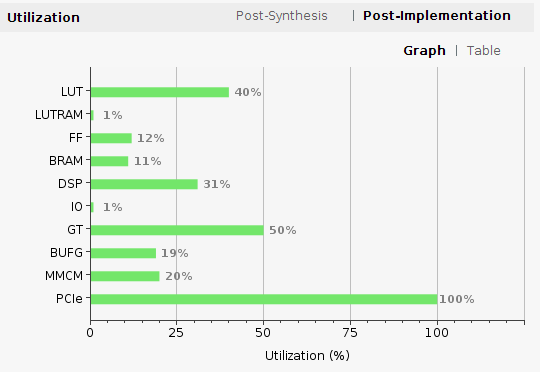
\includegraphics[scale=0.9]{bilder/auslastung1}
\caption{Auslastung auf dem FPGA mit 16-Bit Fixkommazahl und 8 Perceptrons}
\end{figure}\\
Die Auslastung des FPGA für diese Implementierung beträgt in etwa 50\% (siehe Abbildung 4.3), sodass auch 16 Perceptrons parallel geschaltet werden können. Für die bildliche Darstellung in dieser Arbeit wäre dies jedoch ein zu großes Diagramm. 
Die Auslastung für 16 Perceptrons unter MNIST beträgt 90\% der LUT und ist in Abbildung 4.4 veranschaulicht. \\
\begin{figure}[ht]
\centering
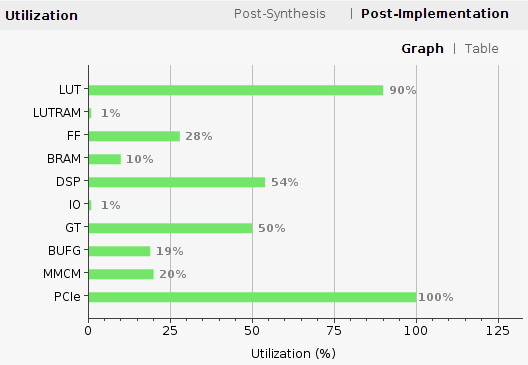
\includegraphics[scale=0.95]{bilder/auslastung2}
\caption{Auslastung auf dem FPGA mit 16-Bit Fixkommazahl und 16 Perceptrons}
\end{figure}\\
Für Datensätze mit mehr Features als MNIST erhöht sich zudem die Auslastung, da jedes Perceptron zwei Koeffizientenvektoren und einen Zwischenpuffer mit einer Länge gleich der Anzahl der Features im Speicher haben muss. Daher können für diese Datensätze keine 16 oder sogar weniger als 8 Perceptrons in das Design eingefügt werden.
%TEsten ob das funktioniert %

 \begin{figure}[ht]
\centering
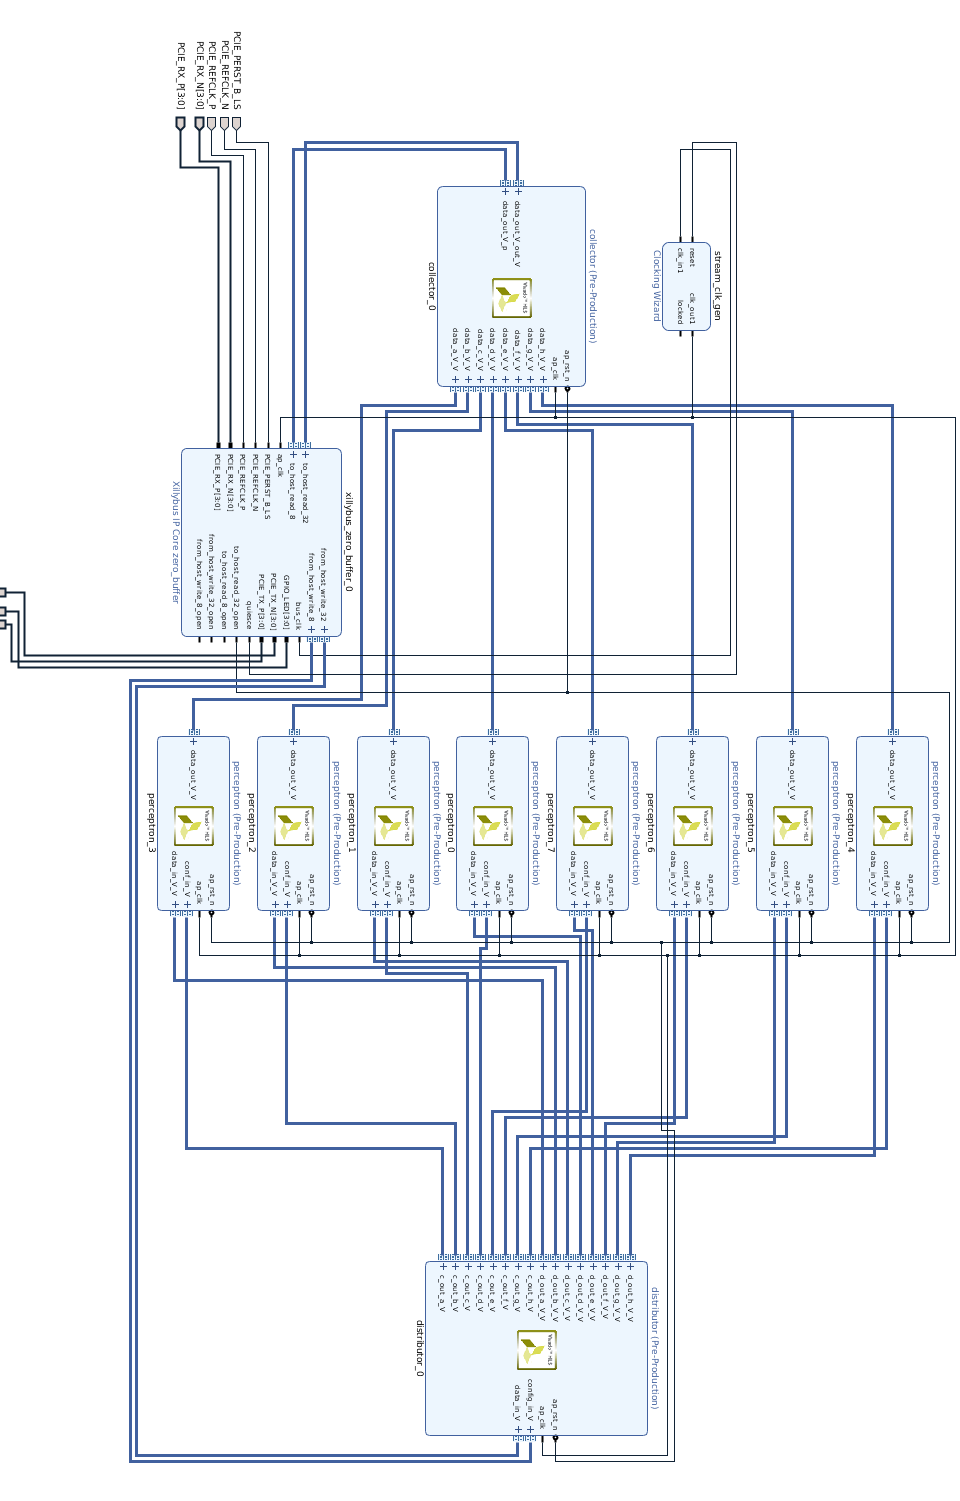
\includegraphics[scale=0.7]{bilder/blockdesign}
\caption{Das Blockdesign auf dem FPGA}
\end{figure}

\chapter{Experimente und Ergebnisse}
In diesem Kapitel werden verschiedene Experimente mit dem FPGA durchgeführt. Zunächst wird gemessen, Wie viel Zeit pro trainiertem Perzeptron für das Training und die Voraussagen auf dem FPGA und einer Implementierung auf dem Hostsystem aufgewendet werden muss. Hierbei wird das Programm auf dem Hostsystem nicht parallelisiert. 
Dann werden beispielhaft Trainingsvorgänge mit verschiedenen Datensätzen durchgeführt, um die Genauigkeit der Vorhersagen zu überprüfen und Ergebnisse der Testvorgänge zu präsentieren.\\
Es werden für die Experimente die Datensätze MNIST \cite{MNIST}, und verwendet.\\
Die Features $\vec f$ des jeweiligen Datensatzes wurden normalisiert, so dass $\forall f \in \vec f\text{ . } f \in [0,1]$. 
\section{Regularisierung}
Mit dem MNIST Datensatz wurden verschiedene Testzyklen zur Regularisierung durchgeführt. Ein Trainingsdurchlauf mit 200 Variablen und 100 Wiederholungen führte zu folgenden Ergebnissen: Hierbei wurde der Datensatz so angepasst, dass alle Variablen die die Ziffer "`3"' darstellen mit "`trifft zu"' und alle anderen Variablen mit "`trifft nicht zu"' markiert wurden.\\\\
\begin{tabularx}{\textwidth}{p{0.16\textwidth}|r|r|r|r|r}
Perceptron & Regularisierungsrate & Lernrate & Batch & Methode & Genauigkeit\\
\hline
a & 0.0 & 0.100098 & 1 & keine & 95.43\%\\
\hline
b & 0.007812 & 0.100098 & 1 & L2 & 95.75\%\\
\hline
c & 0.009766 & 0.100098 & 1 & L2 & 95.75\%\\
\hline
d & 0.5 & 0.100098 & 1 & L2 & 89.9\%\\
\hline
e & 0 & 0.100098 & 1 & L1 & 95.43\%\\
\hline
f & 0.000977 & 0.100098 & 1 & L1 & 95.43\%\\
\hline
g & 0.004883 & 0.100098 & 1 & L1 & 94.38\%\\
\hline
h & 0.009766 & 0.100098 & 1 & L1 & 93.38\%\\
\end{tabularx}


\chapter{Ausblick und Fortsetzung}
Feature Selection mit Daten-Streams\cite{FS}
% Anhang
\appendix
% anhang.tex
\chapter{Weitere Informationen}

% Abbildungsverzeichnis
\listoffigures
\addcontentsline{toc}{chapter}{Abbildungsverzeichnis}
\cleardoublepage
% Literaturverzeichnis
\bibliographystyle{gerplain}
\bibliography{literatur/diplom}
\addcontentsline{toc}{chapter}{\bibname}
% Erklaerung
\thispagestyle{myheadings}
\markboth{}{ERKLÄRUNG}
\addcontentsline{toc}{chapter}{Erklärung}
% erklaerung.tex
\cleardoublepage
\normalsize
Hiermit versichere ich, dass ich die vorliegende Arbeit selbstständig verfasst habe und keine anderen als die angegebenen Quellen und Hilfsmittel verwendet sowie Zitate kenntlich gemacht habe.\\\\
Dortmund, den \today \\\\\\\\
Muster Mustermann
% EOF
\cleardoublepage
\end{document}

